\part{Станки}\label{stanki}

На основе \cp{http://rutracker.org/forum/viewtopic.php?t=3126529}

\copyright\ \prog{Joe Martin}, illustration by \prog{Craig Libuse}

\emph{Tabletop Machining}

A basic approach to making small parts on miniature machine tools

\bigskip

\copyright\ \prog{Джо Мартин}, иллюстрации \prog{Craig Libuse} 

\emph{Настольные станки}

Базовый подход к изготовлению мелких деталей на миниатюрных настольных станках

\clearpage
\chapter{A special note to engineers reading this book}

\section{Machining for engineen and engineering for machinists}

At first glance the subtitle on the cover of this book
could be a bit deceiving. What does tabletop
machining have do with engineering you may ask?
Compare it to a book that has been written about
the ocean. The seas could he described from the
perspective of a young man who has just sailed
around the world in a twenty-five foot sailboat or
by a merchant seaman who has spent his career
aboard a giant ocean liner. Each would have an
entirely different view of what the ocean was all
about. In a stenn, the chap in the small boat would
write ahout surviving broken masts and
mountainous seas while the merchant seaman might
write about seasick passengers. I believe you would
learn more ahout the ocean from the young man in
the small boat, because in a sense he was more
involved in his subject. He was not just on it, he
was in it.

\section{Navigating the seas of machining}

The ocean in this case is the world of machining.
The craftsman using tabletop machine tools is like
the sailor in a small boat, while the professional
machinist with his big CNC shop tools is like the
world-traveling seaman. The process of producing
complex, accurate parts cannot be described by
looking in the window of a quarter million dollar
CNC machine. It would be like a merchant seaman
working in the engine room trying to describe a
stonn in the Atlantic Ocean by telling you how much
extra fuel the ship used. The professional's view of
the subject may be so cluttered with details that it is
difficult to sort the things you really need to know
to sail in rough seas or make good parts. I t is the
craftsman working with small tools, turning the
cranks by hand, who will have the most to tell you
about the real world of working with metal.

\section{looking at engineering from the craftsman's perspedive}

With the aid of computers, parts can easily be drawn
that can't be built. CAD prvgrams allow a designer
to put a perfect .0001 " radius on the inside comer of
a pocket cut in tool steel. Hopefully after reading
this book you will not ask a toolmaker to do it, but
if you do, you'll at least know it is going to cost a
great deal of money to try. Working with metal is
far more difficult than one would imagine. A false
impression is gained by looking at the beautiful yet
inexpensive machined parts that we deal with daily.
They have been produced in very large quantities,
and that five-dollar part you may consider a "ripoff'
could easi ly cost five hundred dollars if you
had to manufacture just one. New engineers will
often think a toolmaker is a failure when the
seemingly simple part they design ends up costing
a thousand dollars to make. Most engineers wi ll
eventually have to deal with the craftsman who tum
their ideas into reality, and in reading this book I
would hope you come away with a new perspective
of what is really involved in producing a machined
part or a product. An alternate subtitle for the book
might have been "Things they should have taught
you in engineering school but didn't". This book
might be considered your textbook for a course
called "Reality WI".

\section{Seeing produdion from the point of view of both
the engineer and machinist}

My perspective on machining could be considered
unique because, in order to survive, I have had to
deal with every aspect of product design from
engineering to prototyping to tooling to
manufacturing to sales. In this book I have tried to
pass along the logic I used to solve the associated
problems. Understanding how a craftsman thinks
and works is an essential part of getting projects
done. Unless you are willing to build your designs
yourself, you are going to have to learn how to deal
with the craftsman who will actually build them.
The more you know about their methods.
personalities and unique problems, the better your
chances are for success. Smooth sailing.

\bigskip\copyright\ Joe Martin

\chapter{About the Joe Martin}

Joe Martin worked in the construction trades after graduating from high school,
but his real love was always building and fl ying radio controlled model
airplanes. When he decided to turn his hobby into a business and start his own
company making components for the radio control industry, he had to learn about
machining and toolmaking on his own. He simply couldn afford to hire anyone else
to set up the tools and make the molds. He has designed and taken to market
numerous products and owned several companies over the years. He began his
association with Sherline Products as an importer of Australi an-built lathes in
the early 1970's. Since then, Joe's company has grown to become the sole
manufacturer and worldwide distributor of Sherline machine tools.

Joe was one of the founders of the sport ofFonnula One model aircraft
competition as well as one of its early champions. His competitive nature seems
to find its way into whatever form of fun he pursues. He has been a winner in
sports from model airplane competition to ocean sai lboat racing and, most
recently, automobile racing.

Never one to be a spectator in life, he has tried and mastered many skills. In
this book, he passes on to you some of his hard-won knowledge about machining.
His down-to-earth s ty le is not hi gh ly polished. In fact, if you could say
that life has put a finish on him, it would probably be described as "" ground
or honed .. . ve ry company making components for the radio control industry, he
had to learn about machining and toolmaking on his own. He simply couldn afford
to hire anyone else to set up the tools and make the molds. He has designed and
taken to market numerous products and owned several companies over the years. He
began his association with Sherline Products as an importer of Australi an-built
lathes in the early 1970's. Since then, Joe's company has grown to become the
sole manufacturer and worldwide distributor of Sherline machine tools.
Joe was one of the founders of the sport ofFonnula One model aircraft
competition as well as one of its early champions. His competitive nature seems
to find its way into whatever form of fun he pursues. He has been a winner in
sports from model airplane competition to ocean sai lboat racing and, most
recently, automobile racing. Never one to be a spectator in life, he has tried
and mastered many skills. In this book, he passes on to acc urate but not slick.
I think his heartfe lt love of good too ls and miniature machining will be
apparent to all who read this book. Working with him these past 25 years is
certainly an experience I would not have wanted to miss.

\bigskip\copyright\ Craig Libuse

\chapter{Dedication}

\note{The photo COII/positioll ahol'e ix ajoillt effort. The photo a/Carl II'OS
taken by his wife Barbara. The photo o/Swall Lake. MOil/alia. a /m'odle spot oj
Carl's, was takeu byfrieud WaYl1e Arll/s/rOllg. The two images were composed ill
PIIO/OShopl by artist £Ioille lolli/IS}

Carl Hammons, my friend and business partner
for thirty years. died September 11 , 1997 as I
was writing this book. We shared thousands of
lunches and coffee breaks over the years we worked
together, and much of the knowledge I have passed
on in this book came from Carl. Carl and I shared
the rare distinction of having been partners not just
once, but twice. We both played different roles in
putting together the product line, and without him
it just isn't going to be as much fun.

When we joined forces for the second time. we had
an agreement that eliminated any need to financially
justify the purchase of a new piece of equipment.
We would buy machines that interested us and find
a job for them later. The laser engraver was a
perfect example of thi s, but now we couldn't get
along without it. It may seem contrary to smart
business practice, but that's the way we did it. I have
no regrets, for we were always the happiest when
we were confronted with a new set of technical
problems. Therefore. I dedicate this book to Carl
Hammons: my business partner, my friend.

\bigskip
I should also credit the English teachers in the
Cranston, Rhode Island school system for forcing a
not-so-willing student enrolled in the "boys general
class" to learn enough about our language to dare to
take on the task of expressing difficult concepts in
simple words. I graduated in 1953. You, the reader,
will be the ultimate judge of their (and my) success
in this undertaking.

\bigskip\copyright\ Joe Martin

\chapter{Safety Rules}
\chapter{Foreword}
\chapter{Introduction}
\chapter{A gallery of machining project photos}

\chapter{SECTION I-GENERAl MACHINING}
\section{Craftsman Profile-Scotty Hewitt ........... 24}
\section{I. Getting information on machining. . . . . . 27}
\section{2. Do you need a lathe. a mill or bOlh? ........ 29}
\section{3. Materials for metalworking .............. 39}
\section{4. Processes for metalworking}
\section{4. I- Heat treating ............ ..• ...... 45}
\section{4.2-Metal fini shes ........... . ........ 46}
\section{4.3-Castings. . . ... .... ..... .... 49}
\section{4.4-----0ther ways 10 form metal .. .. .. . .. .. 5 1}
\section{4.5- Joining metal- Soldering}
\section{and we lding . . . . . . . .. . . .. . .. . 52}
\section{5. Using hand tools and abrasives .......... .. 57}
\section{6. Cutting tools for metalworking}
\section{6. I- General notes on cutting IDols . . 63}
\section{6.2- Cutting tools for both}
\section{the lathe and mill ................... 65}
\section{6.3-Lathe cutting tools ................. 72}
\section{6.4-Culter,S for milling ...... ....... .... 81}
\section{7. Measuring and measurement tools . . . 85}
\section{8. Cool ants and CUlling oils ................ 99}
\section{9. General machining terms . . .. . 101}
\section{10. Machine tool lubrication and maintenancc . 107}

\chapter{SECTION 2-LATHE OPERATIONS}
\section{Craftsman Profile-Jerry Kieffer ..... .. .. .. . 112}
\section{Jerry Kieffer's Flying Pendulum Clock .. . .. 114}
\section{I. Lathe work holding ... .. . .. . .. .. .. . .. . . 115}
\section{2. Lathe operating instnlclions . . . . ......... 121}
\section{3. Tail slock lools and operations . . . . . ...... 141}
\section{4. Ri ser blocks .. . . . . . . . . . . . . ........... 145}
\section{5. Supporting long or thin work . . ... ... . . .. 149}
\section{6. Gelling started in thread cutting. . . . .. 157}
\section{7. Knurled fini shes. . . . . . . . .. .. . ....... 167}
\section{8. Watchmaking and clockmaking tools . ... . 171}
\section{9. Milling operations on a lathe . . . . .. . . . ... 177}

\chapter{SECTION 3-MIll1NG OPERATIONS}
\section{Craftsman Profile- Augie Hiscano . ........ . 180}
\section{I. Holding parts for milling. . . . . . . . . . . . . 183}
\section{2. Mill operating in structions.. . . . ....... . 191}
\section{3. Squaring up a block ...... ........ .. .... 205}
\section{4. The rotary table and index ing attachment ..... 209}
\section{5. Gears and Geartrains ................... 2 19}
\section{6. Accessories for milling}
\section{• Horizontal milling conversion .... . ..... 235}
\section{• Rotary column attachmcnt . . . . . . .. 237}

\chapter{SECTION 4-OTHER MACHINING TOPICS}
\section{Craft sman Profiles-Dan Lutz and Paul White . 242}
\section{I. Setting up a small workshop .... .... .... . 247}
\section{2. Lathe and mill alignment and adj ustments .. 25 1}
\section{3. Enginering drawings . .... .. ............ 259}
\section{4. Frequently asked questions . . . . .. . . . .. . . 265}
\section{5. Making a bus iness o ut of a hobby .. .Joe Martin's}
\section{and Sherline's story ................... 273}
\section{6. Using CNC in a home shop ... ........... 309}

\chapter{SECTION S-PROJECTS AND RESOURCES}
\section{Cra ftsman Profi le-Bob Bres lauer ........... 3 16}
\section{Machini st's tips .......................... 3 18}
\section{I. Plans and projects you can build ........... 3 19}
\section{1. Miniature Tap Handle ... a beginning}
\section{project you can use in your shop ........... 32 1}
\section{2. Mill vise "sofe jaws. . . . . . . . . . . . . . . . 325}
\section{3. Lay ing out a circul ar hole pattern}
\section{fordrilling, a handy skill to learn. . .. . 327}
\section{4. "Millie" ... a small oscillating steam}
\section{engine by Ed Warren, a simple project}
\section{from the pages of Modeltec magazine) ..... . 329}
\section{5. Ordering plans for the Little Ange l}
\section{hit 'n miss engine ... an advanced}
\section{machining project by Bob Shores .......... 333}
\section{2. Contests and awards for tabletop machini sts . . 335}
\section{3. Exploded views and part number li sting}
\section{ Model 4000 and 4400 Lathes .. ......... 340}
\section{ Model 5000 and 5400 Milling machines . . . 341}
\section{ Model 2000 8-Direction Mill Column ..... 342}
\section{ Part number listing ... . ... . ........ . .. 343}
\section{4. A simple RPM gage for your latheor mill ... . 345}
\section{Harold Cli sby and the first Sherline lathe .... . 346}
\section{S. Index ............. .... ...... . . . 347}
\section{ Conversion faclors .. . ... . . .. .. ........ 350}

\chapter{Оборудование}
\clearpage
\section{\odina: станок токарно-винторезный}

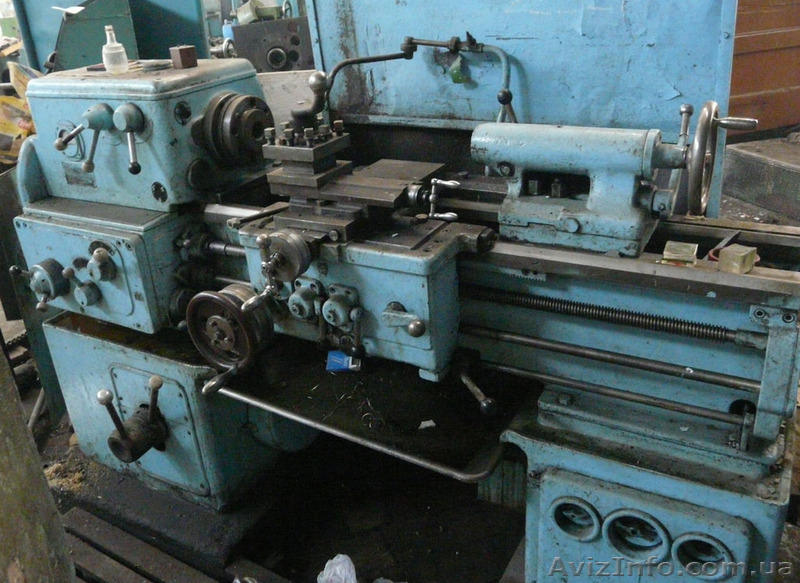
\includegraphics[height=0.5\textheight]{stanki/1A616.jpg}

\subsection{Назначение и области применения}

\subsection{Распаковка и транспортировка}

\subsection{Фундамент станка, монтаж и установка}

\subsection{Подготовка станка к первоначальному пуску}

\subsection{Паспортные данные}

\subsection{Описание основных узлов}

\subsection{Смазка}

\subsection{Первоначальный пуск}

\subsection{Указания по технике безопасности}

\subsection{Настройка}

\subsection{Регулирование}

\subsection{Ведомость комплектации}

